\documentclass[12pt,a4paper]{article}
\usepackage[T1]{fontenc}
\usepackage[utf8]{vietnam}
\usepackage{amsmath}
\usepackage{amssymb}
\usepackage{amsfonts}
\usepackage{enumitem}
\usepackage{fancyhdr}
\usepackage{tikz}
\usepackage{stackrel}
\usepackage{amsthm}
\usepackage{graphicx}
\usepackage{listings}
\usepackage{color}
\definecolor{codegreen}{rgb}{0,0.6,0}
\definecolor{codegray}{rgb}{0.5,0.5,0.5}
\definecolor{codepurple}{rgb}{0.58,0,0.82}
\definecolor{backcolour}{rgb}{0.95,0.95,0.92}
\lstdefinestyle{mystyle}{
    backgroundcolor=\color{backcolour},   
    commentstyle=\color{codegreen},
    keywordstyle=\color{magenta},
    numberstyle=\tiny\color{codegray},
    stringstyle=\color{codepurple},
    basicstyle=\footnotesize,
    breakatwhitespace=false,         
    breaklines=true,                 
    captionpos=b,                    
    keepspaces=true,                 
    numbers=left,                    
    numbersep=5pt,                  
    showspaces=false,                
    showstringspaces=false,
    showtabs=false,                  
    tabsize=2
}
\lstset{style=mystyle}
\usepackage[margin=1.2cm]{geometry}
\title{\LARGE{\textbf{Nhập môn phân tích độ phức tạp thuật toán-21TN}}}
\author{TRẦN MINH HOÀNG-21120075}
\date{} % Ngày không cần hiển thị
\begin{document}
\maketitle
\begin{center}
    \textbf{BÀI TẬP LÝ THUYẾT LẦN 1}
\end{center}


\begin{enumerate}[label=\textbf{Câu 1.\arabic*} ]
    \item Tại sao có thể nói hàm $f(n)=n^{\sqrt{n}}$ thì độ lớn nằm giữa "lớp các hàm đa thức $n^a$(với a>0)" và "lớp các hàm mũ $c^n$ (với c>1)"?
        
    
        \textbf{Giải:} Để chứng minh $\begin{cases}
            f(n)\in \omega(n^a)\\
            f(n)\in o (c^n)
        \end{cases}$
        thì ta cần chứng minh $\begin{cases}
            \lim\limits_{n \to \infty} \frac{f(n)}{n^a}=\infty  \\
            \lim\limits_{n \to \infty} \frac{f(n)}{c^n}=0
        \end{cases}$
        \begin{itemize}[label=$\bullet$] % Sử dụng dấu chấm làm nhãn
            \item $  \lim\limits_{n \to \infty} \frac{f(n)}{n^a}=
            \lim\limits_{n \to \infty} \frac{n^{\sqrt{n}}}{n^a}=
            \lim\limits_{n \to \infty}n^{(\sqrt{n}-a)} =
            \infty^\infty=\infty .\text{ }(1)
            $ 
            \item $\lim\limits_{n \to \infty} \frac{f(n)}{c^n}=
            \lim\limits_{n \to \infty} \frac{n^{\sqrt{n}}}{c^n}=
            \lim\limits_{n \to \infty} \frac{e^{\ln(n^{\sqrt{n}})}}{e^{\ln(c^n)}}=
            \lim\limits_{n \to \infty} \frac{e^{\sqrt{n} \ln(n)}}{e^{n \ln(c)}}=
            e^{\lim\limits_{n \to \infty} (\sqrt{n}\ln(n)-n\ln(c))}.\text{ }(*)\\ \\
            $
            Ta có: $\lim\limits_{n \to \infty} (\sqrt{n}\ln(n)-n\ln(c))=
            \lim\limits_{n \to \infty} \sqrt{n}\ln(n)(1-\frac{n\ln(c)}{\sqrt{n}\ln(n)})=
            \lim\limits_{n \to \infty} \sqrt{n}\ln(n)(1-\frac{\sqrt{n}\ln(c)}{\ln(n)}).\\ \\$
            Lại có:$\lim\limits_{n \to \infty} \frac{\sqrt{n}\ln(c)}{\ln(n)}\stackbin[\infty/\infty]{L'H}{=}
            \lim\limits_{n \to \infty} \frac{\frac{1}{2\sqrt{n}}\ln(c)}{\frac{1}{n}}=
            \frac{\sqrt{n}\ln(c)}{2}=\infty.$\\ \\
            Vậy $\lim\limits_{n \to \infty} (1-\frac{\sqrt{n}\ln(c)}{\ln(n)})=-\infty \Rightarrow
            \lim\limits_{n \to \infty} \sqrt{n}\ln(n)(1-\frac{\sqrt{n}\ln(c)}{\ln(n)})=\infty *(-\infty)=-\infty.$\\ \\
            Hay $\lim\limits_{n \to \infty} (\sqrt{n}\ln(n)-n\ln(c))=-\infty.$\\ \\
            Thay vào (*) $\Rightarrow \lim\limits_{n \to \infty} \frac{f(n)}{c^n}=e^{-\infty}=0.\text{ }(2)$\\ \\
            Vậy từ (1),(2) ta có: 
            $\begin{cases}
                \lim\limits_{n \to \infty} \frac{f(n)}{n^a}=\infty  \\ 
                \lim\limits_{n \to \infty} \frac{f(n)}{c^n}=0 \qed
            \end{cases}$
            
        \end{itemize}
    
        
    \item Đánh giá độ lớn của hàm $f(n)=\frac{\lfloor n^4\log(n)-2n^2+5\rfloor }{\lceil n\sqrt{n^3+1}+10 \rceil} \text{dưới dạng } \Theta(n^c).\\ \\$
        \textbf{Giải:} Đặt $g(n)=n\sqrt{n}\log(n)\\ \\
        \hspace*{1cm}\text{Ta có:} \lim\limits_{n \to \infty} \frac{f(n)}{g(n)}=
        \lim\limits_{n \to \infty} \frac{\frac{\lfloor n^4\log(n)-2n^2+5\rfloor }{\lceil n\sqrt{n^3+1}+10 \rceil}}{n\sqrt{n}\log(n)}
        \simeq \lim\limits_{n \to \infty} \frac{ n^4\log(n)-2n^2+5}{n\sqrt{n}\log(n)(n\sqrt{n^3+1}+10)}\text{(Với n đủ lớn)} \\ \\\hspace*{1.5cm}
        =\lim\limits_{n \to \infty} (\frac{n^2\sqrt{n}}{n\sqrt{n^3+1}+10}-\frac{2\sqrt{n}}{\log(n)(n\sqrt{n^3+1}+10)}+\frac{5}{n\sqrt{n}\log(n)(n\sqrt{n^3+1}+10)}) .$
        \begin{itemize}[label=$\bullet$]
            \item $\lim\limits_{n \to \infty} \frac{n^2\sqrt{n}}{n\sqrt{n^3+1}+10}=\lim\limits_{n \to \infty} \frac{1}{\sqrt{1+\frac{1}{n^3}}+\frac{10}{n^2\sqrt{n}}}=\frac{1}{\sqrt{1+0}+0}=1.$
            \item $\lim\limits_{n \to \infty} \frac{2\sqrt{n}}{\log(n)(n\sqrt{n^3+1}+10)}=\lim\limits_{n \to \infty} \frac{2}{\log(n)(\sqrt{n}\sqrt{n^3+1}+\frac{10}{\sqrt{n}})}=0  .  $
            \item $\lim\limits_{n \to \infty} \frac{5}{n\sqrt{n}\log(n)(n\sqrt{n^3+1}+10)}=0.$
        \end{itemize}
        $\hspace*{1cm}\Rightarrow\lim\limits_{n \to \infty} \frac{f(n)}{g(n)}=1 \in \mathbb{R}  ^{+}.(*)\\ \\$
        Vậy $f(n)\in \Theta(g(n)) \text{ hay } f(n)\in\theta(n\sqrt{n}\log(n)).$
        \item Xét các hàm số $f(x),g(x),h(x)$ xác định và nhận giá trị trên tập số dương,xét tính đúng/sai của mệnh đề sau:Nếu $f(x)g(x)\in \theta(h(x)^2) \text{ và }f(x)\in\Omega(h(x)) \text{thì có }g(x)\in O(h(x)). $\\ \\
        \textbf{Giải:} $f(x)g(x)\in \theta(h(x)^2) \Rightarrow \lim\limits_{n \to \infty}\frac{f(x)g(x)}{h(x)^2} \in \mathbb{R} ^{+}\Rightarrow  \lim\limits_{n \to \infty}[ \frac{f(x)}{h(x)}\frac{g(x)}{h(x)}] \in \mathbb{R} ^{+}(*). \\ \\$
        \hspace*{1cm} Vì $f(x)\in \Omega(h(x))\Rightarrow\lim\limits_{x\to\infty}\frac{f(x)}{g(x)}>0.$
        \begin{itemize}[label=$\bullet$]
            \item Với $\lim\limits_{x \to \infty}\frac{f(x)}{g(x)}=a\in\mathbb{R}^{+}:\\ \\$
                 $\lim\limits_{x \to \infty}\frac{f(x)}{g(x)}\text{ xác định trên }\mathbb{R}^{+}\text{nên thay vào (*) ta được} $
                 $\lim\limits_{x \to \infty}\frac{g(x)}{h(x)}\in \mathbb{R}^{+}\Rightarrow g(x)\in O(h(x)).$  (1)

            \item  Với $\lim\limits_{x \to \infty}\frac{f(x)}{g(x)}=\infty:$\\ \\
            Để (*) đúng thì biểu thức ở trong giới hạn phụ thuộc phải ở dạng vô định và ở đây dạng vô định phải là ở dạng $\infty.0$ do đó ta có thể suy ra được $\lim\limits_{x \to \infty}\frac{g(x)}{h(x)}=0.$\\ \\
            $\Rightarrow g(x)\in O(h(x)).$ Tức là $g(x)\in O(h(x)).$    (2)\\
            \begin{center}
                Từ (1),(2) $\Rightarrow g(x)\in O(h(x)) \Rightarrow $ Mệnh đề đúng.
            \end{center}

        \end{itemize}
    \end{enumerate}
    \begin{enumerate}[label=\textbf{Câu 2.\arabic*} ]
        \item So sánh phí tính toán của hai đoạn code bên dưới:
        \begin{figure}[h] % Chèn ảnh trong môi trường figure, [h] để đặt ảnh ở vị trí hiện tại
            \centering
            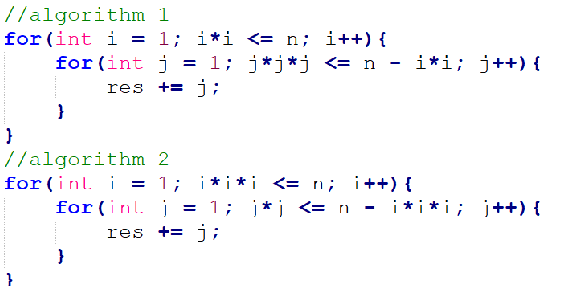
\includegraphics[width=0.5\textwidth]{anh.png} % Thay đường dẫn tới ảnh của bạn ở đây
             % Thêm chú thích cho ảnh
            \label{fig:your_image} % Đặt nhãn cho ảnh để có thể tham chiếu đến trong văn bản
        \end{figure}
        \begin{itemize}[label=$\bullet$]
            \item Xét algorithm 1:
            \begin{center}
                Xét chi phí tính toán của thuật toán bằng số lần thực hiện phép gán $res+=j.$\\
                Vậy từ mã giả ta có được chi phí tính toán của thuật toán trên là :$\sum_{i = 1}^{\lfloor \sqrt{n}\rfloor }\sum_{j = 1}^{\lfloor \sqrt[3]{n-i^2}\rfloor }1.$
            \end{center}
            Vậy khi đó ta cần xem xét chi phí của $f_1(n)=\sqrt[3]{n-1}+\sqrt[3]{n-4}+\sqrt[3]{n-9}+\dots+0 \text{ với } \sqrt{n} \text{ số hạng}.$
            Nhận xét:
            \begin{itemize}[label=$\bullet$]
                \item $f_1(n)\leq\sqrt[3]{n-1}+\sqrt[3]{n-1}+\dots+\sqrt[3]{n-1} (\sqrt{n}\text{ số hạng})=\sqrt{n}\sqrt[3]{n-1}\Rightarrow f_1(n)\in O(n^\frac{5}{6}).$
                \item $f_1(n)\geq \sqrt[3]{n-1}+\sqrt[3]{n-4}+\dots+\sqrt[3]{n-(\frac{\sqrt{n}}{2})^2}\text{ }(\frac{\sqrt{n}}{2}\text{ số hạng})\\ \\
                \hspace*{1cm}\geq \frac{\sqrt{n}}{2}\sqrt[3]{n-\frac{n}{4}}=\frac{\sqrt[3]{6}}{4}\sqrt{n}\sqrt[3]{n}\Rightarrow f_1(n)\in \Omega(n^\frac{5}{6}).$
            \end{itemize}
            Vậy $f_1(n)\in \theta(n^\frac{5}{6}).$ (1)
            \item Xét algorithm 2:
            \begin{center}
                Xét chi phí tính toán của thuật toán bằng số lần thực hiện phép gán $res+=j.$\\
                Vậy từ mã giả ta có được chi phí tính toán của thuật toán trên là :$\sum_{i = 1}^{\lfloor \sqrt[3]{n}\rfloor }\sum_{j = 1}^{\lfloor \sqrt{n-i^3}\rfloor }1.$
            \end{center}
            Vậy khi đó ta cần xem xét chi phí của $f_2(n)=\sqrt{n-1}+\sqrt{n-8}+\dots+0 \text{ với } \sqrt[3]{n} \text{ số hạng}.$
            Nhận xét:
            \begin{itemize}[label=$\bullet$]
                \item $f_2(n)\leq\sqrt{n-1}+\sqrt{n-1}+\dots+\sqrt{n-1} (\sqrt[3]{n}\text{ số hạng})=\sqrt[3]{n}\sqrt{n-1}\Rightarrow f_1(n)\in O(n^\frac{5}{6}).$
                \item $f_2(n)\geq \sqrt{n-1}+\sqrt{n-8}+\dots+\sqrt{n-\frac{n}{8}}\text{ }(\frac{\sqrt[3]{n}}{2}\text{ số hạng})\\ \\
                \hspace*{1cm}>\frac{\sqrt[3]{n}}{2}\sqrt{\frac{7n}{8}}=\frac{\sqrt{14}}{8}\sqrt{n}\sqrt[3]{n}\Rightarrow f_2(n)\in \Omega(n^\frac{5}{6}).$
            \end{itemize}
            Vậy $f_2(n)\in \theta(n^\frac{5}{6}).$ (2)
        \end{itemize}
        Từ (1),(2) ta suy ra độ phức tạp hai thuật toán là như nhau.
        \item Với n nguyên dương, đặt $T_{n}=(\frac{1}{\sqrt{1}}+\frac{1}{\sqrt{2}}+\dots+\frac{1}{\sqrt{n}})(\log(1)+\log(2)+\dots+\log(n)).$ Ước lượng độ lớn của $T_{n}$ theo ký hiệu của $\Theta.$
        \begin{itemize}[label=$\bullet$]
            \item Xét $f(n)=\frac{1}{\sqrt{1}}+\frac{1}{\sqrt{2}}+\dots+\frac{1}{\sqrt{n}}$
            \begin{itemize}[label=$\bullet$]
                \item $f(n) \geq \frac{1}{\frac{\sqrt{n}}{2}}+\dots+\frac{1}{\sqrt{n}}(\frac{n}{2}\text{ số hạng})>\frac{n}{2}\frac{1}{\sqrt{\frac{n}{2}}}=\frac{\sqrt{2}}{2}\sqrt{n}$
                \item $f(n)\leq n\frac{1}{\sqrt{n}}=\sqrt{n}$
            \end{itemize}
            \item Xét $g(n)=\log(1)+\log(2)+\dots+\log(n)$
            \begin{itemize}[label=$\bullet$]
                \item $g(n) \geq \log(\frac{n}{2})+\dots+\log(n)(\frac{n}{2}\text{ số hạng})>\frac{n}{2}\log(n/2)$
                \item $g(n)\leq n\log(n)$
            \end{itemize}
        \end{itemize}
        Vậy khi đó ta có:$\begin{cases}
            \frac{\sqrt{2}}{2}\sqrt{n}\leq f(n)\leq\sqrt{n}\\
            \frac{n}{2}\log(\frac{n}{2})\leq g(n)\leq n\log(n)
        \end{cases}
        \Rightarrow \begin{cases}
            f(n)g(n)\leq n\sqrt{n}\log(n)\Rightarrow T_{n} \in O(n\sqrt{n}\log(n))\\
            f(n)g(n)\geq \frac{\sqrt{2}}{4}n\sqrt{n}\log(\frac{n}{2})\Rightarrow T_{n} \in \Omega(n\sqrt{n}\log(n))
        \end{cases}$
        \begin{center}
            $\Rightarrow T_{n}\in \theta (n\sqrt{n}\log(n))$
        \end{center}
    \end{enumerate}
    
        \begin{enumerate}[label=\textbf{Câu 3}]
        \item Cho dãy số nguyên có n số $a_{1},a_{2},\dots,a_{n} $ mà giá trị mỗi số thuộc tập hợp {0,1,2}.Cần đếm xem có tất cả mấy cách chọn ra cặp chỉ số $(L,R)$ với $1\leq L\leq R\leq n$ sao cho trong dãy con của $a$ xét từ vị trí $L$ đến vị trí $R$ thì có một số nào đó xuất hiện từ 3 lần trở lên.Ví dụ: nếu $a=[0,1,2,2,2] $ thì đáp số là 3, ứng với 3 cách chọn cặp chỉ số $(L,R)=(3,5), (2,5), (1,5).$
        \end{enumerate}
        \begin{enumerate}[label=\textbf{Câu 3.\arabic*},leftmargin=*]
        \item Hãy mô tả cách vét cạn naive cho bài toán trên (dùng mã giả hoặc code C++/Python) và
        đánh giá độ phức tạp tương ứng của thuật toán đó.
        \begin{lstlisting}
            int res=0;
            for(int i=1;i<= n-1;i++){ C[i]
                for(int j=i+1;j<= n;j++){ B[j]
                    int count[]={0,0,0};
                    for(int k=i;k\leqj;k++){ //A[k]
                        count[a[k]]++;
                    }
                    if(count[0]<= 3||count[1]<= 3||count[2]<= 3) res++;
                }
            }
        \end{lstlisting}
        Ta sẽ xét độ phức tạp trong trường hợp xấu nhất đó chính là if luôn thỏa điều kiện.
        Ta xét từng vòng lặp và từ vòng lặp nhỏ nhất  là A(k):
        \begin{itemize}[label=$\bullet$]
            \item Có (j-i+1) phép gán cho giá trị k.
            \item Tiếp theo là gán giá trị cho mảng count.
        \end{itemize}
        $\Rightarrow A(k)=\sum_{k = i}^{j}2=2(j-i+1)  $\\ 
        Ta xét vòng lặp nhỏ tiếp theo là B[j]:
        \begin{itemize}[label=$\bullet$]
            \item có (n-i-1+1) lần gián giá trị cho j.
            \item Mỗi vòng lặp gồm một phép gán cho con trỏ,1 phép gán cho res.
            \item Mỗi vòng lặp phụ thuộc vào i,j ở A.
        \end{itemize}
        $\Rightarrow B(j)=\sum_{j = i+1}^{n}(3+Q(k))=\sum_{j = i+1}^{n}(3+2j-2i+2)  \\ \\
        \hspace*{1.1cm}=\sum_{j = i+1}^{n}(5+2j-2i)=5(n-i-1+1)-2i(n-i)+(n-i)(n+i+1)\\ \\
        \hspace*{1.1cm}=n^2+6n-i(2n+4)+i^2$ \\ 
        Ta xét vòng lặp tiếp theo là C[i]: 
        \begin{itemize}[label=$\bullet$]
            \item có (n-1) phán gán cho giá trị if
            \item Phép gán phụ thuộc i ở B[j]
        \end{itemize}
        $\Rightarrow C[i]=\sum_{i = 1}^{n-1}(B[j]+1)+1=\sum_{i = 1}^{n-1}(n^2+6n-i(2n+4)+i^2+1)+1  \\ \\
        \hspace*{1.1cm}=n^2(n-1)+6n(n-1)-(2n+4)(n-1)\frac{n}{2}+\frac{(n-1)(n-2)}{2}+\frac{(n-1)n(2n-1)}{6}+1\\ \\
        \lim\limits_{n \to \infty}\frac{C[i]}{n^3}=\lim\limits_{n \to \infty}[1-\frac{1}{n^2}+6(\frac{1}{n}-\frac{1}{n^2})-\frac{1}{2}(2+\frac{4}{n})(1-\frac{1}{n})+\frac{(1-\frac{1}{n})(2-\frac{1}{n})}{6}+\frac{1}{n^3}]=\frac{1}{3}\in\mathbb{R}.\\ \\
        \Rightarrow C(n)\in\theta(n^3).$
        \item Bằng cách sử dụng thêm các dãy phụ $x,y,z $ trong đó $x_{i}$ cho biết số giá trị bằng 0 trong dãy từ $a_{1}$ đến $a_{i}$; tương tự $y_{i} $ và $z_{i} $ lần lượt cho biết số giá trị bằng 1 và bằng 2,hãy đề xuất cải thiến cách làm trên thành $O(n^2).$
        \begin{lstlisting}
            int count0[n={0}];
            int count1[n={0}];
            int count2[n={0}];
            for(int i=1;i<= n;i++){
                count0=count0[i-1]+(a[i]==0?1:0);
                count1=count1[i-1]+(a[i]==1?1:0);
                count2=count2[i-1]+(a[i]==2?1:0);
            }
            int res=0;
            for(int i=1;i<= n-2;i++){
                for(int j=i+2;j\<= n;j++){
                    if(count0[j]-count0[i-1]<= 3||count1[j]-count1[i-1]<= 3
                    ||count2[j]-count2[i-1]<= 3) res++;
                }
            }
            return res;
        \end{lstlisting}
        Ta gọi B(n) là phép gán của toàn hàm:
        \begin{itemize}[label=$\bullet$]
            \item có 3 phép gián cố định khai báo mảng.
            \item Mỗi vòng lặp khởi tạo mảng cộng dồn n lần,mỗi lần 3 phép gán tổng là 3n phép gián.
            \item 1 phép gán cố định cho res.
            \item Xét trường hợp xấu nhất của hai vòng for lòng nhau ta gọi A(n) là phép gán của hai vòng for lồng nhau.
        \end{itemize}
        $A(n)=\sum_{i = 1}^{n-2}(1+\sum_{j = i+2}^{n}(1+1))=\sum_{i = 1}^{n-2}(1+2(n-i-1))  \\ \\ 
        \hspace*{1cm}=\sum_{i = 1}^{n-2}(2n-2i-1)=2n(n-2)-(n-2)-(n-2)(n-1)\\ \\
        \hspace*{1cm}=n^2-2n\\ \\$
        Vậy $B(n)=3+3n+1+n^2-2n=n^2+n+4\Rightarrow \lim\limits_{n \to \infty}\frac{P(n)}{n^2}=\lim\limits_{n \to \infty}(1+\frac{1}{n}+\frac{4}{n^2})=1 \in \mathbb{R}.\\ \\
        \Rightarrow P(n)\in \theta(n^2)$
        \item Bằng cách sử dụng nguyên lí Dirichlet,hãy tìm cách cải tiền cách làm trên thành $O(n).\\ \\ $
        \hspace*{1.1cm} Áp dụng nguyên lý Dirichlet,chỉ cần lấy ít nhất 7 phần tử sẽ có ít nhất trong các tập {0,1,2} được lặp lại 3 lần.Vậy thuật toán sẽ là:
        \begin{itemize}[label=$\bullet$]
            \item Đếm số cách L,R có khoảng cách $\geq$ 7.
            \item Loại các trường hợp có khoảng cách 6,5,4,3.
        \end{itemize}
        Số cắp [L,R] thỏa mãn bài toán bằng tổng số đoạn khoảng cách $\geq$ 7 + số trường hợp đếm thêm được.
        \begin{itemize}[label=$\bullet$]
            \item số đoạn có khoảng cách bằng 7 là n-6.
            \item số đoạn có khoảng cách 6 là n-5.
        \end{itemize}
        \begin{center}
            Kiểm tra trong 6 phần tử bằng đoạn mã :int count[3]={0,0,0}
        \end{center}
        \begin{lstlisting}
            for(int i=start;i\leqend;i++){
                count[a[i]]++;
            }
            if(count[0]<= 3||count[1]<= 3||count[2]<= 3) res++;
        \end{lstlisting}
        Ta xét trường hợp xấu nhất sẽ là 1+6.2+1=14.\\ \\ 
        Tương tự với các trường hợp có đoạn khoảng cách là 5,4,3.
        Số đoạn có khoảng cách $\geq$ 7 là:\\ \\
        $(n-6)+(n-7)+(n-8)+\dots+n-n+1=\frac{(n-6)(n-5)}{2}.\\ \\$
        Việc trên đồng nghĩa với việc tính toán trên phụ thuộc vào khoảng cách của 6,5,4,3.\\ \\
        $\Rightarrow \text{Số phép gán }f(n)=(n-5)*14+(n-4)*12+(n-3)*10+(n-2)*8.\\ \\
        \lim\limits_{n \to \infty} \frac{f(n)}{n}=\lim\limits_{n \to \infty}(14(1-\frac{5}{n})+12(1-\frac{4}{n})+10(1-\frac{3}{n})+8(1-\frac{2}{n}))=4 \in \mathbb{R}\\ \\
        \Rightarrow f(n)\in O(n).$
\end{enumerate}
 

\end{document}
